\documentclass[a4paper,11pt]{article}
\usepackage[utf8]{inputenc}
\usepackage[T1]{fontenc}
\usepackage{amsmath}
\usepackage{mathtools}
\usepackage{amsfonts}
\usepackage{amssymb}
\usepackage{graphicx}
\usepackage{multicol}
\usepackage{array}
\usepackage{float}
\usepackage{epstopdf}
\usepackage{caption}
\usepackage{subcaption}
\usepackage{gensymb}
\usepackage[bottom]{footmisc}
\usepackage{appendix}
\usepackage{pdfpages}
\usepackage{todonotes}
\usepackage{mathpazo}
\usepackage{titleps}
\usepackage{color}
\usepackage{xcolor}
\usepackage{colortbl}
\usepackage{siunitx}
\usepackage{pdflscape}
\usepackage{cancel}

\usepackage[skins]{tcolorbox}
\usepackage{sectsty}
\usepackage[arrowmos]{circuitikz}
\usepackage{pgfplots}
\usepackage{blindtext}
\usepackage[inner=2cm,outer=2cm,top=2.5cm,bottom=2.5cm]{geometry}
\usepackage{todonotes}
\usepackage{hyperref}
\usepackage{url}
\usepackage{adjustbox}
\usepackage{tabularx}
\usepackage{booktabs}
\usepackage{fancybox}
\usepackage[tikz]{bclogo}



%For code insertion
%listing
\usepackage{listings}
\usepackage{xcolor}
\definecolor{codegreen}{rgb}{0,0.6,0}
\definecolor{codegray}{rgb}{0.5,0.5,0.5}
\definecolor{codepurple}{rgb}{0.58,0,0.82}
\definecolor{backcolour}{rgb}{0.98,0.98,0.98}
\lstdefinestyle{mystyle}{
    backgroundcolor=\color{backcolour},
    commentstyle=\color{codegreen},
    keywordstyle=\color{blue},
    numberstyle=\tiny\color{codegray},
    stringstyle=\color{codepurple},
    basicstyle=\ttfamily\footnotesize,
    breakatwhitespace=false,
    breaklines=true,
    captionpos=b,
    keepspaces=true,
    numbers=left,
    numbersep=5pt,
    showspaces=false,
    showstringspaces=false,
    showtabs=false,
    tabsize=2
}
\lstset{style=mystyle}



\graphicspath{{figures/}}
\sectionfont{\large}
\subsectionfont{\normalsize}


\newpagestyle{main}{
	\sethead[LELEC2102][][]{LELEC2102}{}{Weeks 11-14}
	\headrule
    \setfoot[][\thepage][]{}{\thepage}{}
}

\newcommand{\horrule}[1]{\rule{\linewidth}{#1}} % Create horizontal rule command with 1 argument of height

%%%%%%%%%%%%%%%%%%%%%%%%%%%%%%%%%%%%%%%%%%%%%%%%%%%%%%%%%%%%%%%%%%%%%%%%%%%%

\begin{document}
\renewcommand{\figurename}{Fig.}

\renewcommand{\thepage}{\arabic{page}}
\setcounter{page}{1}
\pagestyle{main}
\newpage \clearpage

\begin{center}
\begin{LARGE}
LELEC2102: Characterization guidelines
\end{LARGE}
\vspace{0.3cm}
%\textit{TA 1, TA 2}
\end{center}

\section{Classification}

Your objective is to evaluate the performance of the classification in the full chain. To do so, you could reuse part of the work you did for
the report on \emph{Feature vector extraction \& classification}.
% Your focus here will be on the classifier only,
% given a fixed and functional feature vector extraction method. You thus don't need to do any additional analysis on the feature vector
% computation aspects.
Based on the report, you should have chosen a classifier as well as some performance metrics.
We advise you to reuse the same ones for saving time, but you are free to change it.  \\
The most important aspect is that we still expect you to provide classification results both in pure simulation and with the real setup; the comparison between these two results will inform you if:
\begin{itemize}
    \item the classification is bad: a mismatch between simulations and reality would be due to differences between the feature vectors simulated and acquired, the classifier itself, or some data transformation you were not prepared to (e.g. scaling, noise);
    \item the classification is fine: the performances are similar between simulation and real experiments (but if you have a decay in practice, how important is this decay?)
\end{itemize}

To summarise:
\begin{itemize}
    % \item Consider the feature as fixed, don't characterise it.
    \item Characterise your model in simulation on the $5$ classes of ESC-50 dataset (crackling fire, chirping bird, chainsaw, helicopter and handsaw) and study its robustness to transformations.
    \item Always output a prediction, either raw or vector of probability. Don't consider outputting no class for now, this will be for Q2.
    \item Provide the evaluation of your model with the chosen metrics using the full chain (hardware, embedded, crypto, telecom and signal processing). You should do so on at least 50\% of the sounds for each class ($5 \times 20=100$ sounds).
\end{itemize}

To further help you writing this report, you are encouraged to read the
related questions anyone should be able to answer indirectly from its understanding of your report in the \emph{sample questions} pdf available on Moodle.

%%%%%%%%%%%%%%%%%%%%%%%%%%%%%%%%%%%%%%%%
\subsection{Practical measurements}
%%%%%%%%%%%%%%%%%%%%%%%%%%%%%%%%%%%%%%%%
%
The time consuming part is located in the analysis using the full chain.
We suggest you different gradual steps to speed up the process:
%
\begin{itemize}
    \item Write a Python file which browses the dataset and plays each sound one by
    one sequentially.
    It would still require you to push the acquisition button for each sound on a
    row ($500$s$\approx 8$min$20$s).
    \item Modify \emph{auth\_and\_classify} accordingly to output a classification
    result each time a new sound is played.
    An easy way is to make a prediction every 5s as your sounds last 5s,
    but you have the risk to have a drift between the sound playing and the
    acquisitions if one sound is shorter/longer or the acquisition is shorter/longer.
    Another is to synchronize the sound playing with the acquisition
    (probably difficult).
    \item Each sound will have to be associated to a ground truth class and a class predicted by your model.
    If you want to avoid writing this by hand, you could also fill automatically a
    .txt (or any other format) file as the acquisition goes on.
    For the ground truth it would be related to the first file which automatically
    plays the sound. For the acquisition, it would require a small modification
    in \emph{auth\_and\_classify}.
    You finally have to write a Python file which reads your results and displays
    the metrics performances in a figure.
\end{itemize}

\section{Telecommunication}
\subsection{Packet Error Rate}
To obtain the experimental packet error rate (PER) as a function of the signal-to-noise ratio (SNR), one must measure the number of packets incorrectly demodulated by GNU Radio at several SNRs. To facilitate this measurement, we provide you with a script that parses the standard output of GNU Radio and extracts the number of received packets, the number of packet errors, the average estimated SNR as well as the measured CFO.

To use it, you should remove the GUI from GNU Radio (by clicking on the Options block and setting the generate options to 'NO GUI', after having disabled all GUI blocks) and generate the Python script. Then, \textbf{for each SNR level}\footnote{This means that eval\_limesdr\_fpga.py should be run each time you press the B1 button on the MCU. We also suggest you to change the name of the file where the output is redirected, depending on the Tx power used (here, 5 dBm for example).}, run the following command in a terminal:
    \begin{center}
    \textit{python eval\_limesdr\_fpga.py | tee Tx\_5dBm.txt}\\
    \end{center}
This will launch your Python script and redirect the output to the file \textit{Tx\_5dBm.txt}. After the LimeSDR initialisation, you may start sending packet using the radio evaluation mode of the MCU.

Once all packets have been transmitted (at the chosen SNR level), post-process the \textit{Tx\_5dBm.txt} file using the following Python script:
    \begin{center}
    \textit{python read\_file\_for\_CFO\_SNR.py Tx\_5dBm.txt}\\
    \end{center}
The script extracts all the metrics to obtain one point on the PER-SNR curve. Indeed, it prints the average SNR on all packets received, as well as the number of packets received and the number of packet errors. Then, repeat the same steps to obtain a new point on the PER-SNR curve, for another SNR level.

When doing the measurements, please take into account the following remarks:
\begin{itemize}
    \item Use the SMA cable with three 30 dB attenuators. To borrow them, follow the instructions on Moodle.
    \item \textbf{FPGA:} program the FPGA with the bitstream \textit{LimeSDR-Mini\_lms7\_lelec210x\_HW\_1.0\_auto.rpd} provided in FPGA folder of the \texttt{integration} repository. \textit{\textcolor{blue}{This bitstream is different from the one  used in the H4. It uses a 31-taps lowpass filter with a cut-off frequency at $\frac{f_s}{4}$, where $f_s$ is the sampling rate.}}
    \item \textbf{MCU:} set the MCU in radio evaluation mode. Do not forget to increase the number of transmitted packets at each Tx power level, and to decrease the waiting time between each packet transmission\footnote{You can decrease this value in the \textit{eval\_radio.c} file by modifying the HAL delays in the last for loop. For example, set the delays to 10 ms (instead of 500 ms), so that one packet is approximately sent every 20 ms. In this case, sending 1000 packets should take roughly 80 seconds.}. Use a range of Tx powers (between -30 and 15 dBm) that will enable you to reach useful SNRs. Remember that every time the B1 button is pressed, the MCU radio increases the Tx power by 1~dBm.
    \item \textbf{GNU Radio:} use a Rx gain between 60 and 70 dBm. When starting a measurement campaign, \textbf{always} measure the estimated noise power with the chosen Rx gain. Then, set the preamble detection threshold to a value that allows you to detect packets at small SNRs. Be however careful that a too small detection threshold enables the detector to be triggered by noise.
    \textit{Hint: the teaching team used a Rx gain of 70 dB with a detection threshold close to 0.005, which increased when the Tx power increased.}
    \item \textbf{GNU Radio: Disable the hardware preamble detector}, in the LimeSDR FPGA Source block.
\end{itemize}

\subsection{Carrier frequency offset estimation}
You can also extract a histogram of the estimated frequency offsets using the Python script \\ \emph{read\_file\_for\_CFO\_SNR.py} with one of the output files generated for the PER-SNR curve. Ensure that the LimeSDR had enough time to warm up, and use the measurement with the largest SNR.



%%%%%%%%%%%%%%%%%%%%%%%%%%%%%%%%%%%%%%%%%%%%%%%%%%%%%%%%%%%%%%%%%%%%%%%%%%%%%%%%%%%%%%%%%%
\newpage
\begin{comment}
\appendix
\section{Questions}
\subsection{Packet error rate}
Obtain the packet error rate curves as a function of the SNR using the simulation framework. Compare the PER-SNR curve obtained assuming perfect synchronization with the one using all synchronization algorithms. Identify and comment the differences, highlighting their origins with relevant graphs and explanations. Determine the bottleneck in the communication chain. Furthermore, compare these simulated curves with the PER-SNR curve obtained in practice, superimposed on the simulation results. Explain and motivate the differences.

\subsection{Carrier frequency offset estimation}
Discuss the Moose algorithm, based on simulation results and practical measurements. Give and motivate a method to choose the length $N$ of the blocks used by Moose.

Regarding the measurements, obtain a histogram of the carrier frequency offset. What is the shape of the histogram and how can it be linked to $N$?

\subsection{SNR-distance measurements}
Another important aspect of your communication chain is the communication distance that can be achieved. Previously, you identified the required SNR to ensure a desired BER or PER. The next step is therefore to determine the variations of the SNR with the communication distance.

To do so, take some measurements of the estimated SNR (provided in GnuRadio) for several communication distances. Use the antennas with fixed TX and RX gains\footnote{Suggestion: use a RX gain above 50 dB and a TX gain larger than 0 dBm.} and set the preamble detection threshold accordingly. Make sure that the packets are correctly demodulated and average the estimated SNRs over several packets. \textbf{We recommend you to do the measurements outside or in an open area.}


\section{Characterization report}
\textcolor{red}{Add questions in question list, only keep pratical measurement hints.}

\subsection{Packet error rate}
Obtain the packet error rate curves as a function of the SNR using the simulation framework. Compare the PER-SNR curve obtained assuming perfect synchronization with the one using all synchronization algorithms. Identify and comment the differences, highlighting their origins with relevant graphs and explanations. Determine the bottleneck in the communication chain.

Furthermore, compare these simulated curves with the PER-SNR curve obtained in practice, superimposed on the simulation results. Explain and motivate the differences.

\paragraph{Practical measurements} \textcolor{red}{give these details in a separated document?}
To obtain the PER-SNR curve in practice, one must measure the number of packets correctly demodulated at several SNRs. We provide you with a script that can parse the console output of GnuRadio to extract the number of received packets, the number of packet errors, the average estimated SNR as well as the measured CFO.

To use it, you should remove all GUI from GnuRadio (by clicking on the Options block and setting the generate options to 'NO GUI', after having disabled all GUI blocks) and generate the Python script. Then, run the following command in a console:
    \begin{center}
    \textit{python eval\_limesdr\_fpga.py | tee output.txt}\\
    \end{center}
This will launch your Python script and save all console outputs in the file \textit{output.txt}. After the LimeSDR initialisation, you can start sending packet using the MCU radio. At the end, click on enter.

To post-process the \textit{output.txt} file, use:
    \begin{center}
    \textit{python read\_file\_for\_CFO\_SNR.py output.txt}\\
    \end{center}
This should provide all the information required to obtain one point on the PER-SNR curve.

Please take into account the following remarks:
\begin{itemize}
    \item Use the SMA cable with three 30 dB attenuators. \textcolor{red}{how to rent?}
    \item \textbf{FPGA:} program the FPGA with \textcolor{red}{???}
    \item \textbf{MCU:} set the MCU in radio evaluation mode. Do not forget to increase the number of sent packets, as well as decrease the time between each packet sent\footnote{You can decrease this value in the \textit{eval\_radio.c} file by modifying the HAL delays in the last for loop. For example, set the delays to 10 ms (instead of 500 ms), so that one packet is approximately sent every 20 ms. In this case, we measured that sending 1000 packets should take roughly 80 seconds.}. Use a range of TX power that enable you to target the desired SNRs. Remember that every time the B1 button is pressed, the MCU radio will increase the TX power by 1 dBm.
    \item \textbf{GnuRadio:} do not forget to first measure the estimated noise power, with the chosen RX gain. Set the preamble detection threshold to a value that allows you to sense packets at small SNRs. However, a too small detection threshold will be triggered by the noise.
    \textit{Hint: the teaching team used a RX gain of 70 dB with a detection threshold close to 0.005, varying with increasing TX power.}
    \item \textbf{GnuRadio: Disable the hardware preamble detector}, in the LimeSDR FPGA Source block.
    \item For the comparison with the simulated PER curve (with the same modulation parameters, synchronization algorithms and lowpass filter band), remember that the SNR estimated in practice is the SNR right after the lowpass filter and not the one on the decision variable. \textcolor{red}{+updated sim files}
\end{itemize}






\subsection{Carrier frequency offset estimation}
Discuss the Moose algorithm, based on simulation results and practical measurements. Give and motivate a method to choose the length $N$ of the blocks used by Moose.

Regarding the measurements, obtain a histogram of the carrier frequency offset. What is the shape of the histogram and how can it be linked to $N$?

\textit{Hint: you can easily extract all estimated frequency offset and a raw histogram using the Python file \emph{read\_file\_for\_CFO\_SNR.py} with one of the output files generated for the PER-SNR curve. Ideally, take the one with the largest SNR and/or the one where the MCU radio and the LimeSDR had enough time to warm up.}


\subsection{SNR-distance measurements}
Another important aspect of your communication chain is the communication distance that can be achieved. Previously, you identified the required SNR to ensure a desired BER or PER. The next step is therefore to determine the variations of the SNR with the communication distance.

To do so, take some measurements of the estimated SNR (provided in GnuRadio) for several communication distances. Use the antennas with fixed TX and RX gains\footnote{Suggestion: use a RX gain above 50 dB and a TX gain larger than 0 dBm.} and set the preamble detection threshold accordingly. Make sure that the packets are correctly demodulated and average the estimated SNRs over several packets. \textbf{We recommend you to do the measurements outside or in an open area.}


\textcolor{red}{Delete section about path loss exponent. Students can determine it based on their measurements if they want.}

Based on your measurements, determine the path loss exponent. Indeed, assuming the power at the receiver is given by $P_R\:=\:\frac{P_T~G_T~G_R}{L}$, with $P_T$ the power at the transmitter, $G_T$ the gain of the emitter antenna and $G_R$ the gain of the receiver antenna, the path loss $L$ can be extracted\footnote{See LELEC2795 - Communication systems.}. The model for $L$ (in dB) to use is:
\begin{equation*}
    L_{[dB]}\:=\:A \:+\:10~n~\log_{10}(r),
\end{equation*}
with $r$ the communication distance (in meters), $A$ a constant and $n$ the path loss exponent to determine. By expressing the received SNR based on $P_R$, a linear regression can be used to extract the path loss exponent and a constant gathering $P_T$, $G_T$, $G_R$ and $A$.


\newpage
\section{Oral exam questions}

\subsection{BER-PER-SNR}
\begin{itemize}
    \item What is the difference between the input SNR and the SNR on the decision variable? And the SNR after the lowpass filter?
    \item What is a BER? And a PER? What is the link between these two quantities?
    \item How do you measure a PER in practice? Is it possible to measure it if the packet payload is unknown?
\end{itemize}


\subsection{CFO estimation}
\begin{itemize}
    \item Is there a maximal CFO that can be corrected with the Moose algorithm? Where is it coming from? How can it be increased?
\end{itemize}



\newpage
\appendix
\section{Appendix - details PER curve}
\paragraph{Practical measurements}
To obtain the PER-SNR curve in practice, one must measure the number of packets correctly demodulated at several SNRs. Please follow the steps detailed below:

\begin{enumerate}
    \item Use the SMA cable with three 30 dB attenuators, plugged between the MCU radio and the LimeSDR. \textcolor{red}{+ add details about how to rent attenuators...}
    \item \textbf{FPGA:} Program the LimeSDR FPGA with the lowpass filter having 31 taps, that you designed during the Hands-on session 5. \textcolor{red}{NOT SURE ABOUT FILTER!!}
    \item \textbf{MCU:} Program the MCU in radio evaluation mode (by changing \textit{RUN\_CONFIG} in \textit{config.h}). In the \textit{eval\_radio.h} header, make sure to set the minimum TX power level to -15 dBm and the maximum level to -5 dBm. The number of packets should also be increased to 1000. In this case, the MCU radio will send 1000 packets with a payload of 100 bytes, starting at the minimum TX power level. Then, every time you press the B1 button, the power level is increased by 1 dBm and 1000 new packets are sent. By default, packets will be sent every 1 second. Luckily, you can decrease this value in the \textit{eval\_radio.c} file by modifying the HAL delays in the last for loop. For example, set the delays to 10 ms (instead of 500 ms), so that one packet is approximately sent every 20 ms. In this case, we measured that sending 1000 packets should take roughly 80 seconds. \textbf{However, if you notice that your GnuRadio cannot keep demodulating the packets at this speed, you can increase the delays between the packets. You should avoid decreasing the number of sent packets as this will impact the accuracy of the measured packet error rate.}
    \item \textbf{GnuRadio:} The application \textit{eval\_limesdr\_fpga.grc} should be used. However, some changes must be made:
    \begin{itemize}
        %\item First, make sure that all demodulation parameters are the same as in the simulation framework. Namely, you probably changed the length of the sequence used in the Moose algorithm during the H4b session. You should put it back to $N=4$. However, as you noticed, you may not be able to correct any frequency offset in this case, depending on your devices. This is the reason why we suggest you to also perform a fixed frequency offset correction, by slightly modifying the \textit{carrier\_freq} variable in GnuRadio. We encourage you to explain and motivate this fixed frequency offset correction in the question about the CFO histogram. Before going any further, make sure that your communication chain is still working in ideal conditions (large SNR) with this correction. \textcolor{red}{not needed anymore, can keep N=2. Do not hint about fixed CFO then.}
        \item Open \textit{estimate\_noise\_fpga.grc}. Set the RX gain to 70 dB and estimate the noise power with the SMA cable and the 30 dB attenuators plugged-in. (\textit{Hint: it should be close to 1e-6}). Encode this estimated noise power value in \textit{eval\_limesdr\_fpga.grc}.
        \item In \textit{eval\_limesdr\_fpga.grc}, set the RX gain to 70 dB and the preamble detection threshold to 0.003. Moreover, in the LimeSDR FPGA Source block, \textbf{disable the hardware preamble detector}. Make a sanity check by setting the TX MCU radio noise power to -10 dBm and monitoring the number of received packets. You should normally receive all sent packets, with approximately 5 extra packets. These extra packets are received during the initialisation of the LimeSDR because the preamble detection threshold is low. Keep in mind that you will need to discard them later when you will compute the resulting packet error rate.
        \item When the \textit{eval\_limesdr\_fpga.grc} has been parameterized properly, we suggest you to generate a Python file without Graphical User Interface (GUI). This is possible by disabling the QT GUI Sink and QT Gui Range blocks (click on 'd' after having selected the blocks). Then, enable the disabled variable blocks (by clicking on 'e'). Finally, click on the Options block and set the generate options to 'NO GUI'. Generate the Python script (named \textit{eval\_limesdr\_fpga.py}).
    \end{itemize}
    \item Open a terminal and go to the gr-fsk/apps folder. Run the Python script \textit{eval\_limesdr\_fpga.py} with the following command:\\
    \begin{center}
    \textit{python eval\_limesdr\_fpga.py | tee output\_min\_15dBm.txt}\\
    \end{center}
    This will make sure that all the console output of the GnuRadio Python script will be saved in the file \textit{output\_min\_15dBm.txt}. When the LimeSDR has been intialized, click on the B1 button and start sending packets.

    \item When all packets has been received (the blue LED on the MCU is not blinking anymore), click on enter. You now have a file containing the results of all the packets sent at the TX power level of -15 dBm. This file is post-processed using:\\
    \begin{center}
    \textit{python read\_file\_for\_CFO\_SNR.py output\_min\_15dBm.txt}\\
    \end{center}
    This will extract for you the CFO histogram as well as the average SNR and the number of packets received and demodulated properly. You can then deduce the packet error rate at this SNR.

    \item Redo the steps 5 to 6 for another SNR. Do not forget to change the filename and to first launch the \textit{eval\_limesdr\_fpga.py} script, wait for the LimeSDR initialisation and then click on the B1 button.

    \item Compare the practical PER-SNR curve with the simulated one (\textbf{with the same modulation parameters, synchronization algorithms and lowpass filter band}). Remember that the SNR estimated in practice is the input SNR and not the one on the decision variable.
\end{enumerate}

\end{comment}

\section{MCU - Embedded software}
For this part of the characterization, here is a list with key questions to be addressed :
\begin{itemize}
    \item For each of the main functions performed by the MCU, quantify their
        execution time, match them to a part of the current consumption profile
        of the MCU and compute the related energy consumption.
    \item Is the available \textbf{memory} (both volatile and non volatile) a
        limitation (both currently and in the foreseeable future) in the context of
        this project? (\textbf{Hint}: the \textit{Build Analyzer} of your IDE will help you for this.)
    \item Evaluate what would be the impact on the system functionality and
        performance if the following computations would be slower.
        For example, imagine that these computations require twice (or ten times)
        as many cycles as currently.
        \begin{itemize}
            \item Feature vector calculation
            \item Packetizing (including authentication)
            \item Radio transmission
        \end{itemize}
        Based on your evaluation, classify those tasks between \emph{hard
        real-time}, \emph{soft real-time}, and \emph{non real-time}.
    \item Mention and justify your choice of compiler optimization level.
\end{itemize}

\newpage
\section{Power consumption measurements}
We ask you to measure the \textbf{power consumption} profile of the different
components of the embedded system, namely, the \textbf{MCU}, the \textbf{radio},
the \textbf{AFE} and the \textbf{total} consumption of the full system.
To measure the current consumed, you will insert
a \emph{shunt resistor} on the supply line of the device you
measure as in \autoref{fig:measure}. Please make sure you read carefully the last version
of the guide providing details on how to use the boards (see in the folder \texttt{Technical resources} on Moodle).

Practically, you can use the available jumpers as a way of inserting the
resistor. Dedicated jumpers are available on the MCU and the radio boards.
For the AFE, you must use the \textit{AFE\_SUP} selection header where you can
use the connections of the jumper for inserting the resistor.

The value for the shunt resistor is an important parameter of your measurement
setup: if this value is too low or too high, you will not get useful and
accurate measurements. You should be able to justify your choice.
You have access to a large set of resistors during the consultancy sessions.

Finally, we ask you to compare the power consumption of your system with the power that you will be able to harvest
in the future, thanks to the energy harvesting part of the circuit and the PV cells. (\textbf{Hint}: take a look at the data sheet and the characterization of the PV cell that we provided you in the folder \texttt{Technical resources} on Moodle). Does it fit ? Please provide a detailed explanation.

 \begin{figure}[h]
     \centering
     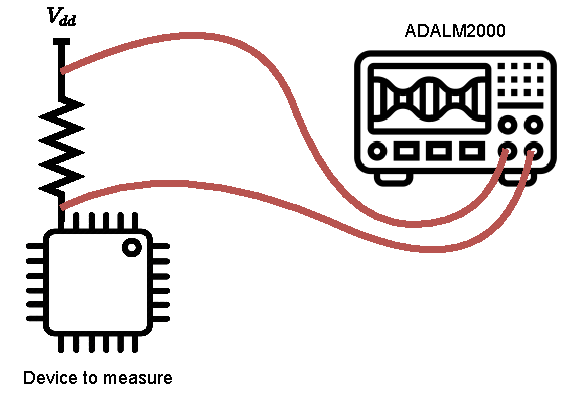
\includegraphics[width=0.35\textwidth]{figs/measure.pdf}
     \caption{%
         How to measure current consumption of a device. You can also use the
         \textit{ADALM2000} to generate a power supply voltage of your choice.
         Stay under the \SI{3.6}{V}, which is the maximum supply voltage of some
         components in the system.
     }
     \label{fig:measure}
 \end{figure}

\begin{bclogo}[couleur = gray!20, arrondi = 0.2, logo=\bcinfo]{Differential probing}
        Contrary to the oscilloscopes of the Marconi lab, the
        \textit{ADALM2000} is a differential oscilloscope, meaning that there
        is no ground on the probe: both probe lines can be at any voltage.
        Therefore, you can use a single channel!\
        However, you must not forget to connect the ground from the \textit{ADALM2000} and the measured device together to align their reference, especially if they are powered by different sources, e.g.\ different computers.
\end{bclogo}
\begin{bclogo}[couleur = gray!20, arrondi = 0.2, logo=\bcattention]{Measure real life conditions}
        Make sure to set up your device for a close to real life usage : Power
        it from an \textbf{external power supply} (as the PV cells would do)
        and not USB. In this mode, you must also make sure to deactivate the
        UART communication in the \texttt{config.h} file to avoid powering the
        ST-link in an undesired way.
\end{bclogo}

\newpage
\section{Crypto - How to perform a side-channel attack}
One of the proposed activities for this semester is about side-channel attacks. We propose you to evaluate the security of the cryptographic operations in your embedded sensor node against the power analysis side-channel attack.
For this purpose, you will use a methodology commonly used in side-channel security evaluation labs: take the role of an attacker and try to perform the best attack possible, that is, the one that uses the least amount of measurements.
To make the evaluation easier, evaluation labs often work on modified versions of the devices to analyze, which allows to performs the evaluation faster (e.g. cryptographic operations are run in a loop, and nothing else is done on the device).

In the following sections, we will show you how to obtain your first side-channel measurements, which we call traces. We then give you hints to mount your first attack, and finally give some practical informations.

\section{General idea}
The underlying idea of a side-channel attack is to exploit data dependent leakages emanating from the device under attack. More concretely, the CMOS circuit used on the MCU consumes power when the output of a logic gate flips from 0 to 1. Therefore, the current consumed by the MCU will be dependent on the data that is manipulated by the MCU. In \autoref{fig:leakage} you can see the current consumption of an MCU operation for different values.\\

\begin{figure}[h]
    \centering
    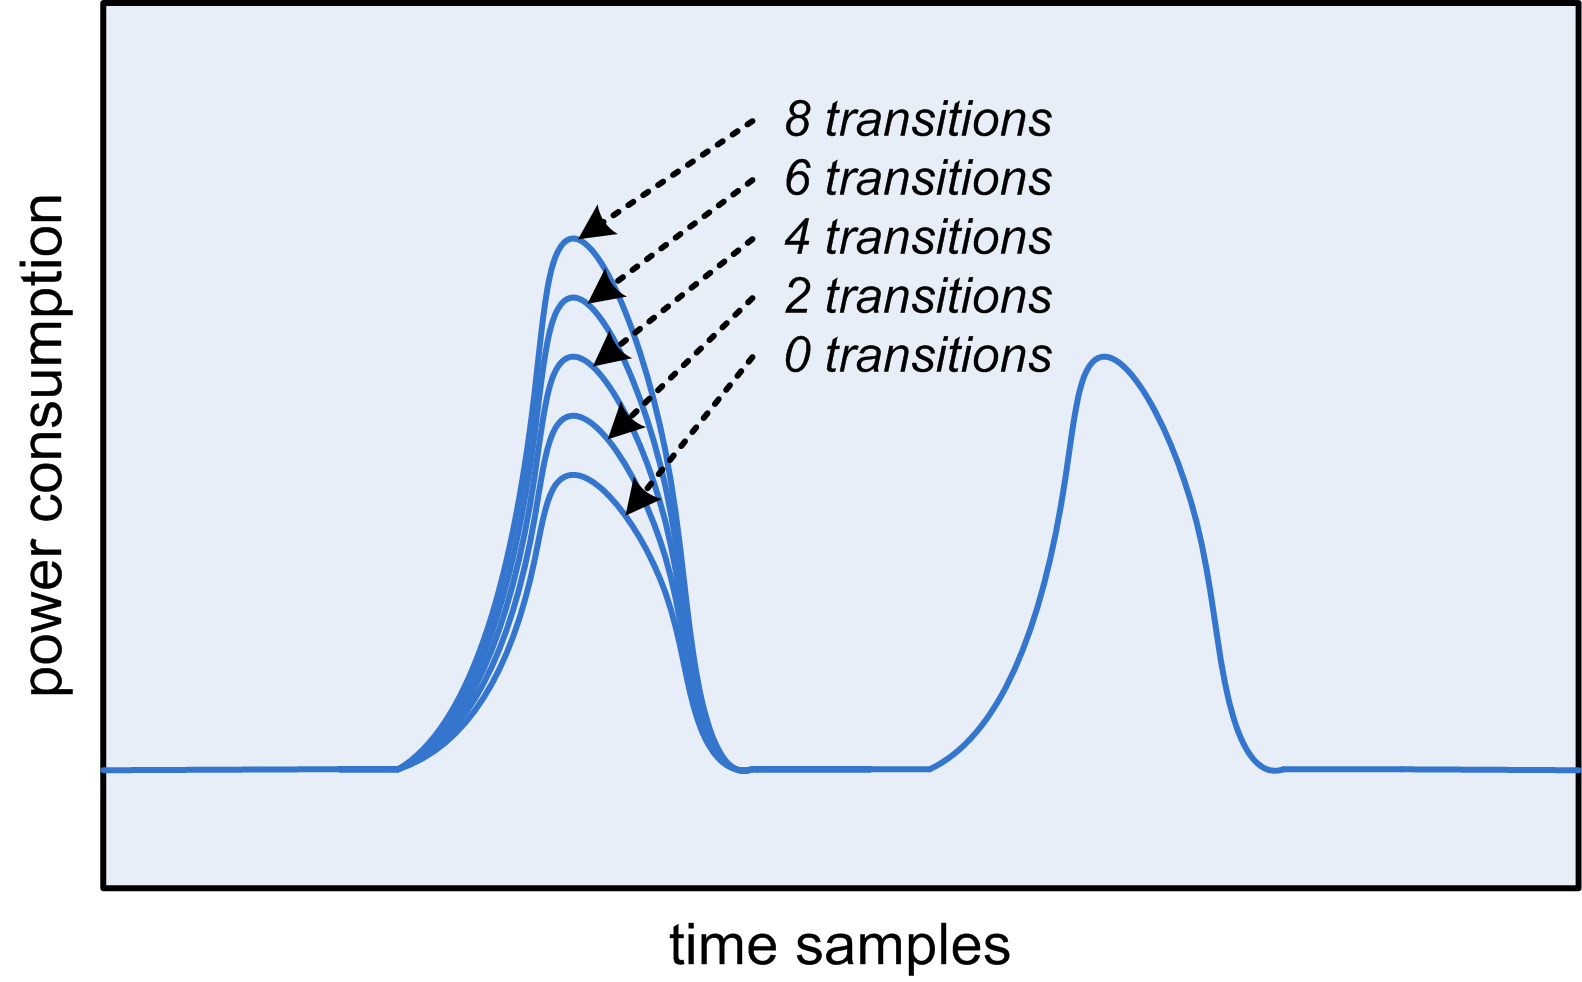
\includegraphics[width=0.5\linewidth]{figs/leakage.png}
    \caption{Power trace illustration for different values of manipulated data}
    \label{fig:leakage}
\end{figure}

To perform a side-channel attack, the attacker (in this case, you) collects measurements of the current consumption and then applies statistical tools to guess a secret value (usually the key for the encryption/authentication). We will show you in the next sections how to perform the current measurements. Then, for the statistical tools, we refer you to the LELEC2760 course material, more specifically, the 6th lecture and 3rd exercice session. All available at the following link : \url{https://perso.uclouvain.be/fstandae/LELEC2760_2022/}. \\

\section{How to prepare your setup}
Similarly to current measurements for the R7 report, you will have to place a shunt resistor on the power line of your MCU and measure the voltage drop on the resistor. You will be using a high performance Picoscope that you can borrow for your measurements.
\begin{bclogo}[couleur = gray!20, arrondi = 0.2, logo=\bcattention]{Picoscope vs ADALM2000}
The picoscope does not have a differential oscilloscope input. Therefore it is mandatory to connect the ground clip of the probe to the ground! Generally, the picoscope is a sensitive and expensive material. Please be cautious and respect at any time the input signal voltage ratings.
\end{bclogo}

\begin{bclogo}[couleur = gray!20, arrondi = 0.2, logo=\bcinfo]{Measurement setup differences from R7 report}
In the context of side-channel meausrements, we are not interested in the absolute value of consumed current, but in the small relative change between measurements. This allows the simplification of the setup in many ways:
\begin{itemize}
    \item Assuming that the 3.3V source connected to the resistor is stable enough, we can connect only one probe and avoid subtracting the result of 2 channels.
    \item The coupling of the oscilloscope can also be changed to AC, improving the vertical resolution of our measurements.
\end{itemize}
\end{bclogo}
When performing side-channel attacks, the attacker needs to synchronize the traces such that each time sample corresponds to the same operation on the MCU, independent of the measurement number. There exists algorithms to perform such alignment from the power traces themselves, but (as commonly used for in evaluation labs), we will skip this step and acquire aligned traces thanks to the use of an additional trigger signal. This trigger signal is a GPIO pin that is set to high just before the beginning of each AES encryption and is set to low after it finishes. This trigger signal will be used as the trigger of the oscilloscope. It is routed on the \textbf{rightmost} (closest to the PCB corner) pin of the \textbf{CTRLS} header on the audio acquisition PCB.

\section{How to acquire traces}
You will have to install a few packages first :
\begin{enumerate}
\item Follow \url{https://www.picotech.com/downloads/linux} to install the Picoscope libraries and software. Note that installing the software automatically installs libraries.
    \item Then install the following python packages: \texttt{numpy scipy matplotlib picosdk}.
\end{enumerate}

Next, read and understand the MCU code that is available on the integration git on the crypto\_DPA branch\footnote{\url{https://forge.uclouvain.be/lelec2102-2103/integration/-/tree/crypto_DPA}}. This code is slightly different from the full project as it only running the AES with per-dertermined plaintexts (again, this is an artificial setup which makes the attack easier to mount for evaluation purposes).

Use the \texttt{collect\_basic.py} acquisition script to collect the traces. You should press the blue button to start encryptions only when the Picoscope is ready. This and the following scripts are located in the \texttt{scripts/sca} folder. This scripts configures the picoscope, you may want to tune this configuration (although the one we give should be sufficient for your first attack).

In order to perform analysis over the traces, you should know the inputs of the AES that were used. To do so, use \texttt{gen\_inputs.py} that replicates the pseudo-random-generator (PRG) implemented on the MCU to derive the inputs (plaintexts) of the AES executions. Make sure that the seed of the PRG is the same on the MCU and in the script. (This PRNG is the reason why it is important that you start the execution of the AES on the MCU only after the picosope is ready to acquire traces: otherwise, the plaintexts generated by the script will not correspond to the acquired traces.)

The remaining file is \texttt{scascope.py} which provides an easy to use interface to the Picoscope library and is used by \texttt{collect\_basic.py}. Some configuration options of the picoscope can be set from here and not from \texttt{collect\_basic.py}.
During acquisition, you should connect the trigger signal as EXT (otherwise you would have to configure two acquisition channels, which wastes precious acquisition memory in the picoscope). You should also aim your signal to fill the vertical range of your scope without overflowing.

\begin{bclogo}[couleur = gray!20, arrondi = 0.2, logo=\bcinfo]{Usage of Picoscope software}
Altough we use scripts to acquire the traces, we advise you to use the Picoscope software to fine tune your setup parameters such as resistor value, vertical range, etc. You can also visualize the trigger signal (for this usage, put in on one of the channels) to learn the timing range you need to sample.

Try to visualize features in the signal: can you visually see patterns in the signal? Is there noise? You can also have a look at the signal in the frequency domain!
\end{bclogo}

\section{Advice for your first attack}
In addition to the classical oscilloscope parameters (vertical and horizontal range), you can play with other variables in this setting : the sampling rate, the vertical resolution. This Picoscope can also do resolution augmenting, that is, averaging multiple samples to obtain higher vertical resolution. As it has a 12 bit ADC, and a maximum sampling rate of 250MS/s, you can reduce the sampling rate for better resolution. We advise you to analyse this tradeoff. (But, for your first attack, the default configuration we gave should work.)

For your first attack, it is necessary to preprocess the traces with a bandpass filter to reduce the noise of unnecessary frequency domains. The \texttt{dpa.py} script contains such a basic filter. Feel free to improve it or remove it for advanced attacks.

As a first side-channel attack, you should aim for the basic \textit{single-bit differential power analysis (DPA)}. You should be able to recover the correct key bytes with 200k traces for the vast majority of the bytes. Then you should optimize your setup. To do so, you can either look at the physical setup, oscilloscope parameters, signal processing, statistical analysis.

The acquisition script can only record 100k traces in the current configuration (due to limited internal memory of the picoscope), but you can make two recordings of the execution (resetting the MCU in-between, but using the same key and PRNG seed), then average the corresponding traces to reduce the physical noise of your measurements (you may also do it with more than 2 recordings).

\section{Booking modalities}
The Picoscopes can be borrowed for at most one day -- they cannot leave the Maxwell building.
In order to book one, you should send an email to \url{gaetan.cassiers@uclouvain.be} \textbf{AND} \url{balazs.udvarhelyi@uclouvain.be}, if possible 2 days in advance. You can retrieve and deposit the Picoscopes at the Maxwell b.125 office.

Do not forget to record your traces in properly labelled and documented files such that you can run and improve the attacks offline, without the Picoscope.

\section{Contest rules}
You were given a MCU project for which you know the source code and can set the key, such that you are in total control of your setup.
During the contest, we will flash the MCU with a binary built from the exact same source code (at -O3 optimization level) but with two differences: the key will be new, and the delay between two AES executions might be modified.\footnote{%
    Maybe you won't be able to acquire 100k traces in a few seconds anymore\dots
}
Your goal will be to recover the secret key as fast as possible.
Finally, a few plaintext/ciphertext pairs will be given to you along with your flashed MCU (e.g., to test if your key guess is correct, or to perform more advanced attacks).


\end{document}
